% Options for packages loaded elsewhere
\PassOptionsToPackage{unicode}{hyperref}
\PassOptionsToPackage{hyphens}{url}
\PassOptionsToPackage{dvipsnames,svgnames,x11names}{xcolor}
%
\documentclass[
  a4paper,
]{report}

\usepackage{amsmath,amssymb}
\usepackage{setspace}
\usepackage{iftex}
\ifPDFTeX
  \usepackage[T1]{fontenc}
  \usepackage[utf8]{inputenc}
  \usepackage{textcomp} % provide euro and other symbols
\else % if luatex or xetex
  \usepackage{unicode-math}
  \defaultfontfeatures{Scale=MatchLowercase}
  \defaultfontfeatures[\rmfamily]{Ligatures=TeX,Scale=1}
\fi
\usepackage{lmodern}
\ifPDFTeX\else  
    % xetex/luatex font selection
\fi
% Use upquote if available, for straight quotes in verbatim environments
\IfFileExists{upquote.sty}{\usepackage{upquote}}{}
\IfFileExists{microtype.sty}{% use microtype if available
  \usepackage[]{microtype}
  \UseMicrotypeSet[protrusion]{basicmath} % disable protrusion for tt fonts
}{}
\makeatletter
\@ifundefined{KOMAClassName}{% if non-KOMA class
  \IfFileExists{parskip.sty}{%
    \usepackage{parskip}
  }{% else
    \setlength{\parindent}{0pt}
    \setlength{\parskip}{6pt plus 2pt minus 1pt}}
}{% if KOMA class
  \KOMAoptions{parskip=half}}
\makeatother
\usepackage{xcolor}
\usepackage[width=150mm,height=238mm,top=27mm]{geometry}
\ifLuaTeX
  \usepackage{luacolor}
  \usepackage[soul]{lua-ul}
\else
  \usepackage{soul}
  
\fi
\setlength{\emergencystretch}{3em} % prevent overfull lines
\setcounter{secnumdepth}{3}
% Make \paragraph and \subparagraph free-standing
\makeatletter
\ifx\paragraph\undefined\else
  \let\oldparagraph\paragraph
  \renewcommand{\paragraph}{
    \@ifstar
      \xxxParagraphStar
      \xxxParagraphNoStar
  }
  \newcommand{\xxxParagraphStar}[1]{\oldparagraph*{#1}\mbox{}}
  \newcommand{\xxxParagraphNoStar}[1]{\oldparagraph{#1}\mbox{}}
\fi
\ifx\subparagraph\undefined\else
  \let\oldsubparagraph\subparagraph
  \renewcommand{\subparagraph}{
    \@ifstar
      \xxxSubParagraphStar
      \xxxSubParagraphNoStar
  }
  \newcommand{\xxxSubParagraphStar}[1]{\oldsubparagraph*{#1}\mbox{}}
  \newcommand{\xxxSubParagraphNoStar}[1]{\oldsubparagraph{#1}\mbox{}}
\fi
\makeatother


\providecommand{\tightlist}{%
  \setlength{\itemsep}{0pt}\setlength{\parskip}{0pt}}\usepackage{longtable,booktabs,array}
\usepackage{calc} % for calculating minipage widths
% Correct order of tables after \paragraph or \subparagraph
\usepackage{etoolbox}
\makeatletter
\patchcmd\longtable{\par}{\if@noskipsec\mbox{}\fi\par}{}{}
\makeatother
% Allow footnotes in longtable head/foot
\IfFileExists{footnotehyper.sty}{\usepackage{footnotehyper}}{\usepackage{footnote}}
\makesavenoteenv{longtable}
\usepackage{graphicx}
\makeatletter
\def\maxwidth{\ifdim\Gin@nat@width>\linewidth\linewidth\else\Gin@nat@width\fi}
\def\maxheight{\ifdim\Gin@nat@height>\textheight\textheight\else\Gin@nat@height\fi}
\makeatother
% Scale images if necessary, so that they will not overflow the page
% margins by default, and it is still possible to overwrite the defaults
% using explicit options in \includegraphics[width, height, ...]{}
\setkeys{Gin}{width=\maxwidth,height=\maxheight,keepaspectratio}
% Set default figure placement to htbp
\makeatletter
\def\fps@figure{htbp}
\makeatother

\makeatletter
\@ifpackageloaded{caption}{}{\usepackage{caption}}
\AtBeginDocument{%
\ifdefined\contentsname
  \renewcommand*\contentsname{Table of contents}
\else
  \newcommand\contentsname{Table of contents}
\fi
\ifdefined\listfigurename
  \renewcommand*\listfigurename{List of Figures}
\else
  \newcommand\listfigurename{List of Figures}
\fi
\ifdefined\listtablename
  \renewcommand*\listtablename{List of Tables}
\else
  \newcommand\listtablename{List of Tables}
\fi
\ifdefined\figurename
  \renewcommand*\figurename{Figure}
\else
  \newcommand\figurename{Figure}
\fi
\ifdefined\tablename
  \renewcommand*\tablename{Table}
\else
  \newcommand\tablename{Table}
\fi
}
\@ifpackageloaded{float}{}{\usepackage{float}}
\floatstyle{ruled}
\@ifundefined{c@chapter}{\newfloat{codelisting}{h}{lop}}{\newfloat{codelisting}{h}{lop}[chapter]}
\floatname{codelisting}{Listing}
\newcommand*\listoflistings{\listof{codelisting}{List of Listings}}
\makeatother
\makeatletter
\makeatother
\makeatletter
\@ifpackageloaded{caption}{}{\usepackage{caption}}
\@ifpackageloaded{subcaption}{}{\usepackage{subcaption}}
\makeatother

\ifLuaTeX
  \usepackage{selnolig}  % disable illegal ligatures
\fi
\usepackage{bookmark}

\IfFileExists{xurl.sty}{\usepackage{xurl}}{} % add URL line breaks if available
\urlstyle{same} % disable monospaced font for URLs
\hypersetup{
  pdftitle={Further Quantitative Methods},
  pdfauthor={Kevin Lingfeng Li},
  colorlinks=true,
  linkcolor={blue},
  filecolor={Maroon},
  citecolor={Blue},
  urlcolor={Blue},
  pdfcreator={LaTeX via pandoc}}


\title{Further Quantitative Methods}
\usepackage{etoolbox}
\makeatletter
\providecommand{\subtitle}[1]{% add subtitle to \maketitle
  \apptocmd{\@title}{\par {\large #1 \par}}{}{}
}
\makeatother
\subtitle{Companian to the series: Introduction to Political Economics}
\author{Kevin Lingfeng Li}
\date{}

\begin{document}
\maketitle

\renewcommand*\contentsname{Table of contents}
{
\hypersetup{linkcolor=}
\setcounter{tocdepth}{1}
\tableofcontents
}

\setstretch{1.25}
\chapter*{Preface}\label{preface}
\addcontentsline{toc}{chapter}{Preface}

This book is one of the 3 \textbf{mathematical-companian-guides} of the
part of a series: \textbf{Introduction to Political Economics}. These
companian guides are meant to ensure that one has the proper
mathematical training prior to studying Political Economics:

\begin{enumerate}
\def\labelenumi{\arabic{enumi}.}
\tightlist
\item
  \textbf{Quantitative Methods} introduces the essential mathematical
  concepts that are essential for studying Political Economics. Topics
  include algebra, single variable calculus, and probability and
  statistical theory.
\item
  \textbf{Further Quantitative Methods} (This Book) expands on the
  topics taught in the previous book. These topics are not
  ``essential'', but it is highly recommended to have some grasp of
  these topics. Topics include linear algebra and multivariate calculus.
\item
  \textbf{Introductory Proofs and Analysis} is a high-level introduction
  to proofs in mathematics. This is not essential for studying Political
  Economics, but having a strong idea behind proofs is quite useful for
  more advanced Microeconomic Models that are used in the study of
  Political Economics.
\end{enumerate}

This book, Further Quantitative Methods, is a collection of mathematical
and statistical topics that I consider to very useful, although not
absolutely essential, before instruction of Political Economics. This
book assumes a strong understanding of high-school level algebra, as
well as the algebra and calculus topics from \emph{Quantitative
Methods}. In this book, we first discuss topics in linear algebra,
before moving on to multivariate calculus.

\part{Introductory Linear Algebra}\label{introductory-linear-algebra}

\chapter{Matrices}\label{matrices}

\section{Matrix Operations}\label{matrix-operations}

topics 3.2-3.3

\section{Inverse Matrix}\label{inverse-matrix}

\section{Simple Linear Systems of Square
Matrix}\label{simple-linear-systems-of-square-matrix}

\section{Elementary Row Operations and Reduced Row Echelon
Form}\label{elementary-row-operations-and-reduced-row-echelon-form}

\section{Theorems on Matrix
Invertibility}\label{theorems-on-matrix-invertibility}

\section{Determinant of a Matrix}\label{determinant-of-a-matrix}

\section{Linear Systems of Invertible Square
Matrix}\label{linear-systems-of-invertible-square-matrix}

\chapter{General Linear Systems}\label{general-linear-systems}

\section{Geometric Insight of a 2-Dimensional
Plane}\label{geometric-insight-of-a-2-dimensional-plane}

\section{K-dimensional Flats}\label{k-dimensional-flats}

\section{Solving Lienar Systems of
Equations}\label{solving-lienar-systems-of-equations}

\section{Solution Sets and Linearity}\label{solution-sets-and-linearity}

\section{Analysing Solution Sets with the
Rank}\label{analysing-solution-sets-with-the-rank}

\part{Basics of Probability and
Statistics}\label{basics-of-probability-and-statistics}

\chapter{Basic Probability}\label{basic-probability}

See
\href{https://kevinli03.github.io/politicaleconomy/maths.pdf}{Mathematical
Methods for Political Economy} for more detailed explanations.

\section{Sets and Set Operators}\label{sets-and-set-operators}

A \textbf{set} is the collection of objects, while the \textbf{elements}
of the set are the specific objects within a set. A capital letter is
used to represent a set, for example, set \(A\). A lowercase letter
represents an element within the set. For example, element \(a\) is a
part of set \(A\).

There are a few different set operators that are important to
understand.

An \textbf{intersection} of sets \(A\) and \(B\), formally notated
\(A \cap B\), indicates the elements that are both within \(A\) and
\(B\) at the same time.

\begin{itemize}
\tightlist
\item
  For example, if \(A = \{1,2,3\}\) and \(B = \{2,3,4\}\), then
  \(A \cap B = \{2, 3\}\), since those are the elements that are
  contained in both \(A\) and \(B\) at the same time.
\end{itemize}

A \textbf{union} of sets \(A\) and \(B\), formally notated as
\(A \cup B\), indicates elements that are in either \(A\), \(B\), or
both \(A\) and \(B\).

\begin{itemize}
\tightlist
\item
  For example, if \(A = \{1,2,3\}\) and \(B = \{2,3,4\}\), then
  \(A \cap B = \{1,2, 3,4\}\).
\item
  \(A \cup B = A + B -A \cap B\). We subtract \(A \cap B\) since that
  part is counted twice in both \(A\) and \(B\), so we need to get rid
  of it once to avoid over-counting.
\end{itemize}

The \textbf{complement} of set \(A\) is everything that is not in \(A\),
but still within the universal set. The complement is denoted as \(A'\)
or \(A^c\).

\begin{itemize}
\tightlist
\item
  For example, if the universal set contains \(\{1,2,3,4,5\}\), and
  \(A = \{1,2\}\), then \(A' = \{3,4,5\}\)
\end{itemize}

A \textbf{subset} \(A\) has all its elements belonging to another set
\(B\). This is notated \(A \subset B\).

\begin{itemize}
\tightlist
\item
  For example, if \(A = \{1,2\}\), and \(B = \{1,2,3\}\), then \(A\) is
  a subset of \(B\) since all of \(A\)'s elements belong to set \(B\) as
  well.
\end{itemize}

\section{Basic Properties of
Probability}\label{basic-properties-of-probability}

\textbf{Kolmogrov's Axioms} are the key properties of probability:

\begin{enumerate}
\def\labelenumi{\arabic{enumi}.}
\tightlist
\item
  For any event \(A\), the probability of \(A\) occurring is between 0
  and 1.
\item
  The probability of all events in the sample space \(S\) is 1.
  Mathematically: \(Pr(S) = 1\). The sample space is the set of all
  possible events.
\item
  If we have a group of mutually exclusive events
  \(A_1, A_2, ... , A_k\), then the probability of those events all
  occurring is the sum of their probabilities. Mathematically,
  \(Pr \left( \bigcup A_i \right) = \sum Pr(A_i)\)

  \begin{itemize}
  \tightlist
  \item
    Note: mutually exclusive events are events that cannot occur at the
    same time together.
  \end{itemize}
\end{enumerate}

Other important properties to note include:

\begin{itemize}
\item
  \(Pr(A') = 1 - Pr(A)\) - the probability of the complement of \(A\),
  is equal to 1 minus the probability of \(A\)
\item
  \(Pr(A \cup B) = Pr(A) + Pr(B) - Pr(A \cap B)\) - this is because of a
  property of unions, as shown in section 2.2
\end{itemize}

\section{Joint and Conditional
Probability}\label{joint-and-conditional-probability}

\textbf{Joint Probability} is the probability of two or more events
occurring simultaneously. The joint probability of events \(A\) and
\(B\) is notated \(Pr(A \cap B)\).

For example, in a deck of cards, \(A\) could be the event of drawing an
ace, and \(B\) could be the event of drawing a spade. Thus,
\(Pr(A \cap B)\) would be the probability of drawing a card that was
both an ace and a spade.

\textbf{Conditional Probability} is the probability of one event
occurring, given another has already occurred. Probability of event
\(A\), given event \(B\) has occurred, is notated as \(Pr(A|B)\)

To calculate the conditional probability, we use the following formula:

\[
Pr(A|B) = \frac{Pr(A \cap B)}{Pr(B)}
\]

\section{Bayes' Theorem}\label{bayes-theorem}

\textbf{Bayes' Theorem} states the following relationship is true:

\[
Pr(A|B) = \frac{Pr(B|A) \times Pr(A)}{Pr(B)}
\]

Each part of Bayes' Theorem has a name. They are commonly referenced, so
it is useful to know their names:

\begin{itemize}
\item
  \(Pr(A|B)\) is the \ul{conditional} probability
\item
  \(Pr(B|A)\) is the \ul{posterior} probability
\item
  \(Pr(A)\) is the \ul{prior} probability
\item
  \(Pr(B)\) is the \ul{marginal} probability
\end{itemize}

\chapter{Basic Statistics}\label{basic-statistics}

See \href{https://kevinli03.github.io/maths.pdf}{Essential Mathematics
for Political Economy} for more detailed explanations.

\section{Random Variables}\label{random-variables}

Random variables are variables that represent unobserved events that
have some randomness - a set of potential outcomes, with each outcome
having a probability of occurring.

For example, if you flip a coin 10 times, and count the number of heads
you get, you could get 5 heads, 6 heads, 4 heads, or any amount between
0 and 10. We are not sure what will happen - however, some outcomes are
more likely than others, because of the probabilities associated with
each outcome.

There are two types of random variables:

\begin{itemize}
\item
  \textbf{Discrete Random Variables} are random events which have a
  distinct number of outcomes. For example, rolling a dice has 6
  outcomes.
\item
  \textbf{Continuos Random Variables} are random events which have an
  infinite amount of outcomes. For example, my drive to work tomorrow
  could take 5 minutes, 5.123 minutes, 5.234237847 minutes, and so
  on\ldots{} there is no distinct outcomes since you can continuously
  subdivide the gaps between outcomes by adding more decimal points.
\end{itemize}

\section{Distributions and Probability Density
Functions}\label{distributions-and-probability-density-functions}

Random variables are often called distributions - because there are a
distribution of outcomes, with associated probabilities for each
outcome. We can actually graph this - put potential outcomes on the
\(x\) axis, and the probability that each outcome occurs on the \(y\)
axis.

For example, take this probability distribution of a die - there are 6
sides that you could land on, and each has an equal probability of
occurring:

\begin{center}
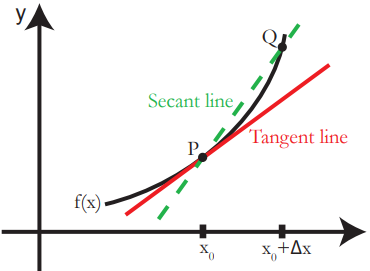
\includegraphics[width=0.5\textwidth,height=\textheight]{figures/1/2.1.png}
\end{center}

The \textbf{probability mass/density function} \(f(y)\) takes a
potential outcome of an event as an input, and outputs the respective
probability.

For example, the probability mass/density function of a dice is
\(f(y) = 1/6\). This is because every outcome \(y\) has the same
probability of occurring: \(1/6\). So \(f(1), f(2)... = 1/6\).

\section{Expectation and Variance}\label{expectation-and-variance}

Expectation and Variance are two ways we can summarise the distributions
of random variables.

The \textbf{expectation}, often called the expected value or mean, is
the best guess of an outcome of a random variable, given no other
information except its distribution. We notate expected value of a
variable \(Y\) as either \(E[Y]\), \(\bar{Y}\), or \(\mu\).

The expected value for discrete variables is calculated by multiplying
each outcome value by its associated probability, then doing that for
all outcomes, and summing everything together. In other words, it is a
weighted average of the outcomes, with the weights being the probability
of each outcome.

\[
E[Y] = y_1 \times f(y_1) + y_2 \times f(y_2)... = \sum [y_j \times f(y_j)]
\]

For a continuous random variable, it is a little more complicated. This
is because continuous variables have an infinite number of potential
outcomes. For example, if you drive to school, your driving time could
be 23 minutes, or 23.12 minutes, or 23.123324 minutes\ldots{} basically,
an infinite amount. As a result, we have to alter the expected value
formula a little:

\[
E[Y] = \int\limits_{-∞}^∞ y \times f(y)dy
\]

\textbf{Variance} \(\sigma^2\) is a measure of how spread out our
distribution is. Variance basically measures how far values are, on
average, from the mean of the variable. Mathematically:

\[
Var(X) = \sigma^2 = \frac{1}{n} \sum (X-\mu)^2 = E[(X - \mu)^2]
\]

Where \(\sigma^2\) is the variance, \(n\) is the number of observations,
and \(\mu\) is the mean of \(X\)

\textbf{Standard Deviation} \(\sigma\) is the square root of variance
\(\sigma^2\)

\section{Normal Distribution and T
Distribution}\label{normal-distribution-and-t-distribution}

A \textbf{normal distribution} is in the shape of a bell curve. The mean
\(\mu\), mode, and median are all the same value at the centre, and the
distribution is symmetrical on both sides. The figure below shows the
typical shape of a normal distribution

\begin{center}
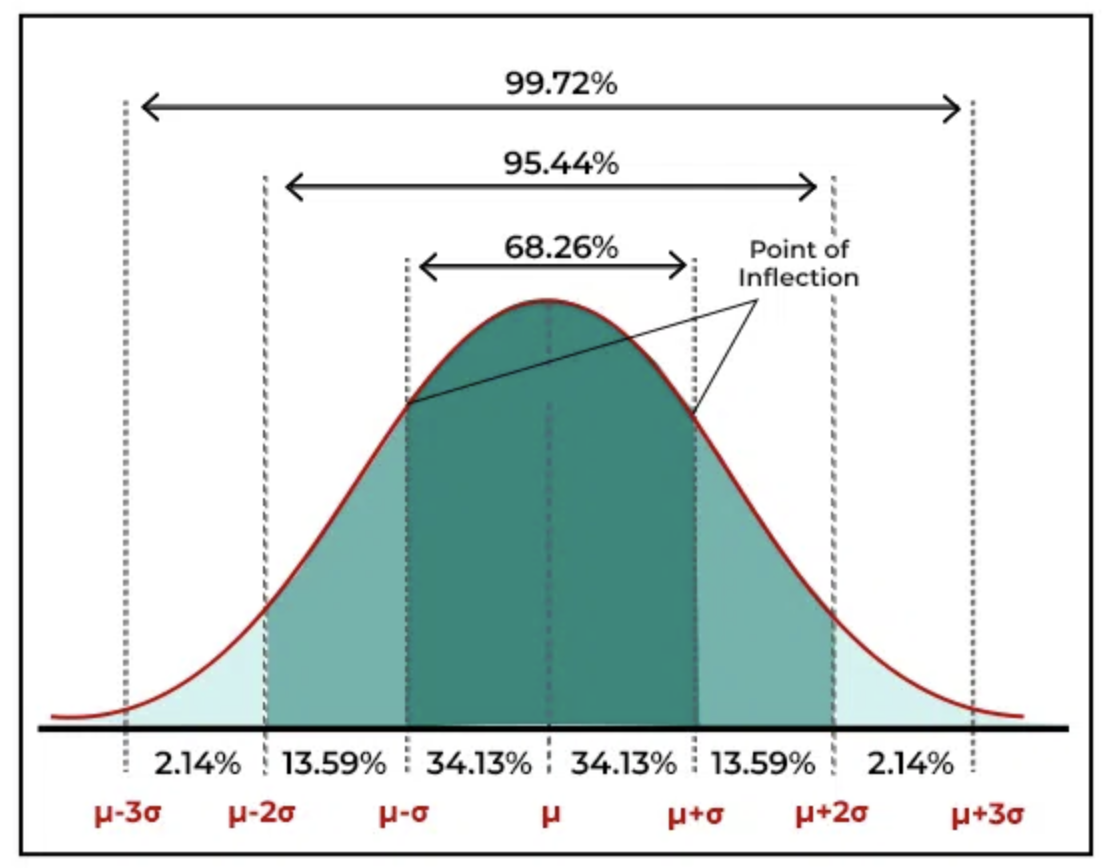
\includegraphics[width=0.6\textwidth,height=\textheight]{figures/1/2.2.png}
\end{center}

All Normal Distributions, as shown in the image above, follow the
68-95-99.7 rule:

\begin{itemize}
\item
  Within one standard deviation \(\sigma\) of the mean \(\mu\), lies
  68.26\% of the total area under the curve
\item
  Within 2 standard deviations \(2 \sigma\) of the mean \(\mu\), lies
  95.44\% of the total area under the curve
\item
  In fact, any amount of standard deviations \(\sigma\), including
  decimals, is related to a specific percent of total area under the
  curve, for all normal distributions.
\end{itemize}

This is important, because the \ul{area under the distribution curve is
the probability}. Thus, the normal distribution tells us there is a
relationship between the standard deviation and the probability of an
action occurring.

Any normal distribution can be described with 2 features: mean \(\mu\)
and variance \(\sigma^2\) in the following form:
\(X \sim \mathcal{N}(\mu, \sigma^2)\). For example,
\(X \sim \mathcal{N} (30, 4)\) means a normal distribution with mean 30
and variance 4.

The T distribution is a distribution very similar to the shape and size
of the normal distribution, however, generally has thicker tails and a
lower peak. The key difference is that t-distributions are defined with
only one parameter - degrees of freedom \(DF\).

\section{Covariance and Correlation}\label{covariance-and-correlation}

In political economy, we are often interested in the relationship
between two variables. For example, are oil producers more likely to be
democratic? Are more educated voters more likely to turn out and vote?
The relationship between two features, also called correlation, is the
extent to which they tend to occur together.

\begin{itemize}
\item
  A positive correlation/relationship is when we are more likely to
  observe feature \(Y\), if feature \(X\) is present
\item
  A negative correlation/relationship is when we are less likely to
  observe feature \(Y\), if feature \(X\) is present
\item
  No correlation/relationship is when we see feature \(X\), that does
  not tell us anything about the likelihood of observing \(Y\)
\end{itemize}

We can also visualise these graphically:

\begin{center}
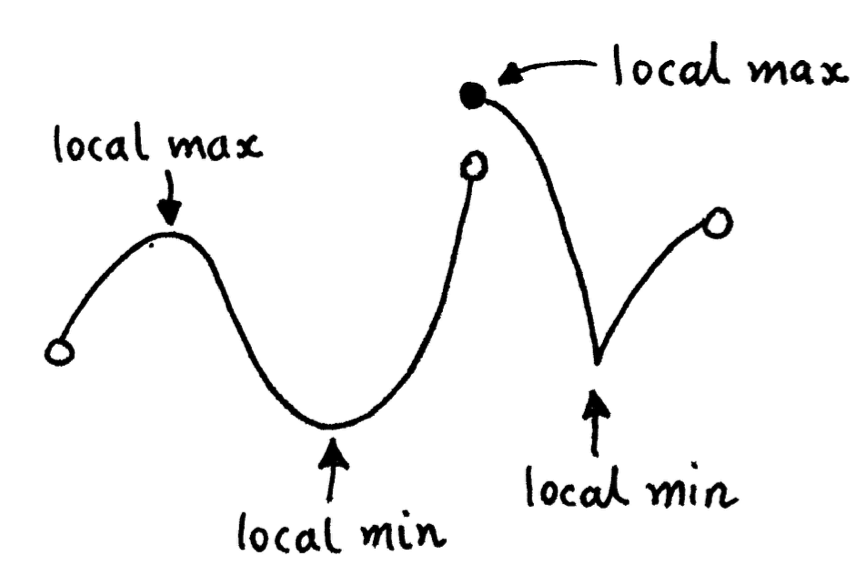
\includegraphics[width=0.8\textwidth,height=\textheight]{figures/1/3.1.png}
\end{center}

\textbf{Covariance} is a way to measure the relationship between two
variables. Covariance is the extent that \(X\) and \(Y\) vary together.
Mathematically:

\[
Cov(X,Y) = \sigma_{XY} = \frac{1}{n} \sum (X_i - \bar{X})(Y_i - \bar{Y})
\]

Or more simply:

\begin{itemize}
\item
  In our data, we have many different pairs of data points
  \((X_i, Y_i)\)
\item
  \(X_i\) is some value of \(X\), and \(\bar{X}\) is the mean of \(X\).
  Same goes for \(Y_i\) and \(\bar{Y}\)
\item
  Thus, \(X_i - \bar{X}\) is the distance between any point \(X_i\) and
  the mean \(\bar{X}\). Same goes for \(Y_i - \bar{Y}\)
\item
  \(n\) is the number of observations (data points) in our data
\end{itemize}

We can interpret the sign of the covariance: if it is positive, we have
a positive relationship. if it is negative, we have a negative
relationship. However, \ul{we cannot interpret the numerical value of
the covariance}.

To do that, we have to find the \textbf{correlation coefficient}. We
calculate this by taking the covariance, and dividing it by the product
of the standard deviation of \(X\) and the standard deviation of \(Y\).
Mathematically:

\[
Corr(X,Y) = r = \frac{Cov(X,Y)}{\sigma_X \sigma_Y}
\]

The correlation coefficient is always between -1 and 1.

\begin{itemize}
\item
  The direction is the same as the covariance - if the coefficient is
  positive, then we have a positive relationship, vice versa.
\item
  If the correlation coefficient is closer to -1 or 1, it means a strong
  correlation. If the correlation is closer to 0, then it is a weak
  correlation
\end{itemize}

\section{Best Linear Predictor}\label{best-linear-predictor}

While the correlation coefficient tells us the strength of a
correlation, it does not say anything about the magnitude of the
relationship. For example, if \(X\) increases by one unit, how much does
\(Y\) increase by? The correlation coefficient does not say.

\begin{itemize}
\tightlist
\item
  In a linear model, the \(X\) variable is considered the
  \textbf{explanatory} or \textbf{independent} variable, while the \(Y\)
  is the \textbf{response} or \textbf{dependent} variable.
\end{itemize}

Magnitude is quite an important concept. After all, even if two values
are very highly correlated, if an increase of one unit in \(X\) only
leads to a miniscule increase in \(Y\), this relationship might not be
very important for understanding the world.

A way to estimate the magnitude of the relationship between \(X\) and
\(Y\) is the \textbf{best linear predictor.} The best linear predictor
is a best fit line for the data, that takes the form of a linear
equation: \(Y = \alpha + \beta X\).

In this equation, the \(\beta\) term in the best fit line is the slope
of the linear equation. Essentially, it tells us for every increase in
one unit of \(X\), how much do we expect \(Y\) to increase by?

\begin{itemize}
\tightlist
\item
  We can interpret the sign of \(\beta\): a positive \(\beta\) is a
  positive relationship, a negative \(\beta\) is a negative
  relationship, and \(\beta = 0\) is no relationship.
\item
  We can also interpret the magnitude of \(\beta\): as \(X\) increases
  by 1 unit, \(Y\) is expected to increase by \(\beta\) units.
\end{itemize}

The Best Linear Predictor is a form of Linear Regression, the primary
topic we will cover in the next two chapters.




\end{document}
